


%%%%%%%%%%%%%%%%%%%%%%%%%%%%%%%%%%%%%%%%%
% Beamer Presentation
% LaTeX Template
% Version 1.0 (10/11/12)
%
% This template has been downloaded from:
% http://www.LaTeXTemplates.com
%
% License:
% CC BY-NC-SA 3.0 (http://creativecommons.org/licenses/by-nc-sa/3.0/)
%
%%%%%%%%%%%%%%%%%%%%%%%%%%%%%%%%%%%%%%%%%

%----------------------------------------------------------------------------------------
%	PACKAGES AND THEMES
%----------------------------------------------------------------------------------------

\documentclass{beamer}

\mode<presentation> {

% The Beamer class comes with a number of default slide themes
% which change the colors and layouts of slides. Below this is a list
% of all the themes, uncomment each in turn to see what they look like.

%\usetheme{default}
%\usetheme{AnnArbor}
%\usetheme{Antibes}
%\usetheme{Bergen}
%\usetheme{Berkeley}
%\usetheme{Berlin}
%\usetheme{Boadilla}
%\usetheme{CambridgeUS}
%\usetheme{Copenhagen}
%\usetheme{Darmstadt}
\usetheme{Dresden}
%\usetheme{Frankfurt}
%\usetheme{Goettingen}
%\usetheme{Hannover}
%\usetheme{Ilmenau}
%\usetheme{JuanLesPins}
%\usetheme{Luebeck}
%\usetheme{Madrid}
%\usetheme{Malmoe}
%\usetheme{Marburg}
%\usetheme{Montpellier}
%\usetheme{PaloAlto}
%\usetheme{Pittsburgh}
%\usetheme{Rochester}
%\usetheme{Singapore}
%\usetheme{Szeged}
%\usetheme{Warsaw}

% As well as themes, the Beamer class has a number of color themes
% for any slide theme. Uncomment each of these in turn to see how it
% changes the colors of your current slide theme.

%\usecolortheme{albatross}
\usecolortheme{beaver}
%\usecolortheme{beetle}
%\usecolortheme{crane}
%\usecolortheme{dolphin}
%\usecolortheme{dove}
%\usecolortheme{fly}
%\usecolortheme{lily}
%\usecolortheme{orchid}
%\usecolortheme{rose}
%\usecolortheme{seagull}
%\usecolortheme{seahorse}
%\usecolortheme{whale}
%\usecolortheme{wolverine}

\setbeamertemplate{footline} % To remove the footer line in all slides uncomment this line
%\setbeamertemplate{footline}[page number] % To replace the footer line in all slides with a simple slide count uncomment this line

\setbeamertemplate{navigation symbols}{} % To remove the navigation symbols from the bottom of all slides uncomment this line
}

\usepackage{graphicx} % Allows including images
\usepackage{booktabs} % Allows the use of \toprule, \midrule and \bottomrule in tables
\usepackage{etex}
\usepackage{listings}
\usepackage{pgfplots}
%\usepackage{pygmentize}
%\usepackage{minted}
\usepackage[all]{xy}
\usepackage[font=Times, timeinterval= 59]{tdclock}
\usetikzlibrary{positioning}
\usetikzlibrary{shapes.geometric}
\usepackage{blkarray}

%----------------------------------------------------------------------------------------
%	TITLE PAGE
%----------------------------------------------------------------------------------------

\title{Verifiable Homomorphic Tallying for the Schulze Vote Counting Scheme} % The short title appears at the bottom of every slide, the full title is only on the title page

%\author{Mukesh Tiwari} % Your name

\author[shortname]{Mukesh Tiwari\inst{1} \and Dirk Pattinson\inst{1} 
\and Thomas Haines \inst{2}}
\institute{\inst{1} Research School of Computer Science, 
	Australian National University, Australia \and 
    \inst{2} Department of Mathematical Sciences,
       Norwegian University of Science and Technology, Norway}
                      
%\author[Mukesh Tiwari]{Mukesh Tiwari\\{Dirk Pattinson\newline 
%Thomas Haines}}
%\institute[ANU] % Your institution as it will appear on the bottom of every slide, may be shorthand to save space
%{
%Australian National University \\[1em] Research School of Computer Science% Your institution for the title page
%%\medskip
%%%\textit{john@smith.com} % Your email address
%}
%\date[\today]{\today \\ {Joint work with Dirk Pattinson, and Thomas Haines}}
%\date{22 November, 2018} % Date, can be changed to a custom date


\begin{document}


\defverbatim[colored]\genmargin{
\begin{lstlisting}[language=haskell, basicstyle=\ttfamily\scriptsize, commentstyle=\color{red}\ttfamily]
Fixpoint M (n : nat) (c d : cand) : Z :=
      match n with
      | 0%nat => marg c d
      | S n' =>
        Z.max 
           (M n' c d) 
           (maxlist (map 
           (fun x : cand => 
        	  Z.min (marg c x) (M n' x d)) cand_all))
end.

\end{lstlisting}}

\defverbatim[colored]\lstf{
\begin{lstlisting}[language=haskell, basicstyle=\ttfamily\scriptsize, commentstyle=\color{red}\ttfamily]
{- Propositional Path -}
Inductive Path (k: Z) : cand -> cand -> Prop :=     
| unit c d : marg c d >= k -> Path k c d    
| cons  c d e : 
   marg c d >= k -> Path k d e -> Path k c e.
   
{- Notion of winner at prop level -}    
Definition wins_prop (c: cand) := 
  forall d : cand, exists k : Z,     
   Path k c d /\ 
   (forall l, Path l d c -> l <= k).   

{- Notion of loser at prop level -}
Definition loses_prop (c : cand) := 
  exists k: Z, exists  d: cand,     
   Path k d c /\ 
   (forall l, Path l c d -> l < k).
\end{lstlisting}}

\defverbatim[colored]\lsts{
\begin{lstlisting}[language=haskell, basicstyle=\ttfamily\scriptsize]

Definition marg_lt (k : Z) (p : (cand * cand)) :=
	Zlt_bool (marg (fst p) (snd p)) k.

Definition W (k:Z) (p:cand * cand -> bool) (x:cand * cand) :=     
 andb (marg_lt k x)       
 (forallb (fun m => 
   orb (marg_lt k (fst x, m)) 
       (p (m, snd x))) cand_all).
 
Definition coclosed (k:Z) 
 (f:(cand * cand) -> bool) :=     
  forall x, f x = true -> W k f x = true.   
 
    
\end{lstlisting}}


\defverbatim[colored]\lstt{
\begin{lstlisting}[language=haskell,commentstyle=\color{red}\ttfamily, basicstyle=\ttfamily\scriptsize ]
{- Type level Path -}
Inductive PathT (k: Z) : cand -> cand -> Type :=   
| unitT :forall c d, 
   marg c d >= k -> PathT k c d   
| consT :forall c d e,
   marg c d >= k -> PathT k d e -> PathT k c e.

{- Notion of winner at type level -} 
Definition wins_type c := 
 forall d : cand, existsT (k : Z),     
  (PathT k c d * existsT f,       
  f (d, c) = true /\ coclosed (k + 1) f)).   

{- Notion of loser at type level -}
Definition loses_type (c : cand) := 
 existsT (k : Z) (d : cand),     
  (PathT k d c * existsT f,       
  f (c, d) = true /\ coclosed k f)).
  
Lemma wins_type_prop : forall c, wins_type c -> wins_prop c.  
Lemma wins_prop_type : forall c, wins_prop c -> wins_type c.
\end{lstlisting}
}


\defverbatim[colored]\lstfourth{
\begin{lstlisting}[language=haskell, basicstyle=\ttfamily\tiny, commentstyle=\color{red}\ttfamily]
Inductive State: Type :=     
| partial: (list ballot * list ballot)  -> (cand -> cand -> Z) -> State     
| winners: (cand -> bool) ->  State.

{- Different states of counting -}
Inductive Count (bs : list ballot) : State -> Type :=     
| ax us m : us=bs -> (forall c d, m c d = 0) -> 
   Count bs (partial (us, []) m)            
| cvalid u us m nm inbs : 
   Count bs (partial (u :: us, inbs) m) -> 
   (forall c, u c > 0) -> 
   (forall c d : cand, 
     (u c < u d -> nm c d = m c d + 1) /\                                           
     (u c = u d -> nm c d = m c d)     /\                                    
     (u c > u d -> nm c d = m c d - 1)) ->                                
   Count bs (partial (us, inbs) nm)
| cinvalid u us m inbs : 
   Count bs (partial (u :: us, inbs) m) ->
   (exists c, u c = 0) -> Count bs (partial (us, u :: inbs) m)     
| fin m inbs w (d : (forall c, (wins_type m c) + (loses_type m c))):
   Count bs (partial ([], inbs) m) -> 
   (forall c, w c = true <-> (exists x, d c = inl x)) ->         
   (forall c, w c = false <-> (exists x, d c = inr x)) ->         
   Count bs (winners w).    
\end{lstlisting}
}


\defverbatim[colored]\lstfifth{
\begin{lstlisting}[language=haskell, basicstyle=\ttfamily\tiny]
Theorem schulze_winners: forall (bs : list ballot),     
  existsT (f : cand -> bool) (p : Count bs (winners f)), True.
  
V: [A1 B2 C3,..], I:  [], M: [AB:0 AC:0 BC:0]
---------------------------------------------
V: [A1 B2 C3,..], I:  [], M: [AB:1 AC:1 BC:1]
---------------------------------------------
             . . .
---------------------------------------------
V: [A2 B3 C1], I:  [], M: [AB:2 AC:0 BC:6]
------------------------------------------
V: [], I: [], M: [AB:3 AC:-1 BC:5]
----------------------------------
winning: A
   for B: path A -> B of strenght 3, 4-coclosed set:
     [(A,A),(B,A),(B,B),(C,A),(C,B),(C,C)]
   for C: path A -> B -> C of strenght 3, 4-coclosed set:
     [(A,A),(B,A),(B,B),(C,A),(C,B),(C,C)] 
losing: B
   exists A: path A -> B of strength 3, 3-coclosed set:
     [(A,A),(B,A),(B,B),(C,A),(C,B),(C,C)]
losing: C
   exists A: path A -> B -> C of strength 3, 3-coclosed set:
     [(A,A),(B,A),(B,B),(C,A),(C,B),(C,C)]  
\end{lstlisting}
}

\defverbatim[colored]\lstsix{
\begin{lstlisting}[language=haskell, basicstyle=\ttfamily\tiny]
Inductive HState: Type :=
 | hpartial: (list eballot * list eballot)  -> (cand -> cand -> Z) -> HState 
 | hdecrypt: (cand -> cand -> Z) -> HState
 | winners: (cand -> bool) -> HState.	
\end{lstlisting}
}

\defverbatim[colored]\lstseven{
\begin{lstlisting}[language=haskell, basicstyle=\ttfamily\tiny]
Inductive HCount (bs : list eballot) : HState -> Type :=
 | ax us (m : cand -> cand -> Z) (ev : cand -> cand -> Z): 
      us = bs -> (forall c d, enc 0 (ev c d) = m c d) -> 
      HCount bs (hpartial (us, []) m)

 | cvalid u us m nm inbs (v : cand -> cand -> Z) (p : Zkp u v) 
          (b : cand -> cand -> Z)
          (ev : cand -> cand -> Z) :
          HCount bs (hpartial (u :: us, inbs) m) -> 
          (check_zkp u v (p : Zkp u v) = true) -> 
          (forall c d, enc (b c d) (ev c d) = v c d) ->
          valid b ->
          (forall c d, nm c d = m c d  + u c d) ->
          HCount bs (hpartial (us, inbs) nm)
  
 | cinvalid u us m inbs (v : cand -> cand -> Z) (p : Zkp u v) 
            (b : cand -> cand -> Z)
            (ev : cand -> cand -> Z) : 
            HCount bs (hpartial (u :: us, inbs) m) ->
            (check_zkp u v p = true) -> 
            (forall c d, enc (b c d) (ev c d) = v c d) -> 
            invalid b  -> 
            HCount bs (hpartial (us, u :: inbs) m)

 
\end{lstlisting}
}
\defverbatim[colored]\lsteight{
\begin{lstlisting}[language=haskell, basicstyle=\ttfamily\tiny]

| cderypt inbs m ev dm : HCount bs (hpartial ([], inbs) m) -> 
           (forall c d, enc (m c d) (ev c d) = dm c d) ->
           HCount bs (hdecrypt dm)

 | fin dm w (d : (forall c, (wins_type dm c) + (loses_type dm c))) :
        HCount bs (hdecrypt dm) -> 
        (forall c, w c = true <-> (exists x, d c = inl x)) ->
        (forall c, w c = false <-> (exists x, d c = inr x)) ->
        HCount bs (winners w).	
        
\end{lstlisting}
}

\defverbatim[colored]\matvalid{
\begin{lstlisting}[language=haskell, basicstyle=\ttfamily\tiny]
 
   Definition matrix_ballot_valid (p : pballot) :=
      (forall c d : cand, In (p c d) [-1; 0; 1]) /\
      (exists f : A -> nat,
          forall c d : A,
          (p c d = 1 <-> (f c < f d)%nat) /\
          (p c d = 0 <-> f c = f d) /\ 
          (p c d = -1 <-> (f c > f d)%nat))
         
    Lemma matrix_ballot_valid_dec : 
        forall p : pballot, {matrix_ballot_valid p} +
                            {~matrix_ballot_valid p}.
 \end{lstlisting}
}   

\defverbatim[colored]\lstnineth{
\begin{lstlisting}[language=haskell, basicstyle=\ttfamily\tiny]
V: [A3 B1 C2 D4,..], I: [], M: [AB:0 AC:0 AD:0 BC:0 BD:0 CD:0]
--------------------------------------------------------------
V: [A1 B0 C4 D3,..], I: [], M: [AB:-1 AC:-1 AD:1 BC:1 BD:1 CD:1]
----------------------------------------------------------------
V: [A3 B1 C2 D4,..], I: [A1 B0 C4 D3], M: [AB:-1 AC:-1 AD:1 BC:1 BD:1 CD:1]
---------------------------------------------------------------------------
                     . . .
----------------------------------------------------------------------
V: [A1 B3 C2 D4], I: [A1 B0 C4 D3], M: [AB:2 AC:2 AD:8 BC:5 BD:8 CD:8]
----------------------------------------------------------------------
V: [], I: [A1 B0 C4 D3], M: [AB:3 AC:3 AD:9 BC:4 BD:9 CD:9]
-----------------------------------------------------------
winning: A
  for B: path A --> B of strength 3, 4-coclosed set: 
    [(B,A),(C,A),(C,B),(D,A),(D,B),(D,C)]
  for C: path A --> C of strength 3, 4-coclosed set:
    [(B,A),(C,A),(C,B),(D,A),(D,B),(D,C)]
  for D: path A --> D of strength 9, 10-coclosed set:
    [(D,A),(D,B),(D,C)]
losing: B
  exists A: path A --> B of strength 3, 3-coclosed set:
    [(A,A),(B,A),(B,B),(C,A),(C,B),(C,C),(D,A),(D,B),(D,C),(D,D)]
losing: C
  exists A: path A --> C of strength 3, 3-coclosed set:
    [(A,A),(B,A),(B,B),(C,A),(C,B),(C,C),(D,A),(D,B),(D,C),(D,D)]
losing: D
  exists A: path A --> D of strength 9, 9-coclosed set:
    [(A,A),(A,B),(A,C),(B,A),(B,B),(B,C),(C,A),(C,B),(C,C),(D,A),(D,B),
     (D,C),(D,D)]
\end{lstlisting}
}       

\defverbatim[colored]\lsttenth{
\begin{lstlisting}[language=haskell, basicstyle=\ttfamily\tiny]

Inductive Path (k: Z) : cand -> cand -> Prop :=     
| unit c d : marg c d >= k -> Path k c d    
| cons  c d e : 
   marg c d >= k -> Path k d e -> Path k c e.  
        
\end{lstlisting}
}

\defverbatim[colored]\marginstable{
\begin{lstlisting}[language=haskell, basicstyle=\ttfamily\scriptsize]

      Lemma iterated_marg_fp: forall (c d : cand) (n : nat),
             M n c d <= M (length cand_all) c d.
        
\end{lstlisting}
} 
\defverbatim[colored]\lsteleven{
\begin{lstlisting}[language=haskell, basicstyle=\ttfamily\scriptsize]

Lemma iterated_marg_fp: forall (c d : cand) (n : nat),
      M n c d <= M (length cand_all) c d.

Lemma wins_prop_iterated_marg (c : cand) : wins_prop c ->
      forall d, M (length cand_all) d c <= M (length cand_all) c d.

Lemma iterated_marg_wins_type (c : cand) : (forall d,
      M (length cand_all) d c <= M (length cand_all) c d) ->
      wins_type c.

        
\end{lstlisting}
} 

\defverbatim[colored]\lsttwelve{
\begin{lstlisting}[language=haskell, basicstyle=\ttfamily\scriptsize]
Theorem schulze_winners: forall (bs : list ballot),     
  existsT (f : cand -> bool) (p : Count bs (winners f)), True.
  

\end{lstlisting}
}



\defverbatim[colored]\lstthirteen{
\begin{lstlisting}[language=haskell, basicstyle=\ttfamily\tiny]
Definition plaintext := Z.
Definition ciphertext := (Z * Z)%type. 


    (* ballot is plain text value *)
Definition ballot := cand -> cand -> plaintext.
    (* eballot is encrypted value *)
Definition eballot := cand -> cand -> ciphertext.

    

Inductive EState : Type :=
    | epartial : (list eballot * list eballot) ->
                 (cand -> cand -> ciphertext) -> EState
    | edecrypt : (cand -> cand -> plaintext) -> EState
    | ewinners : (cand -> bool) -> EState.


\end{lstlisting}
}

\defverbatim[colored]\lstfourteen{
\begin{lstlisting}[language=haskell, basicstyle=\ttfamily\tiny]
	(* This function will be realized by Elgamal Encryption.
 		Enc_Pk (m, r) = (g^r, g^m * h^r) *)
Variable encrypt_ballot : Pubkey -> ballot ->  eballot.

    (* This function will be realized by Elgamal Decryption
       which takes encrypted message (c1, c2), private key
       and outputs the plaintext message *)
Variable decrypt_ballot : Prikey -> eballot -> ballot.

    (* This function takes encrypted ballot and returns
       permuted encrypted ballot with zero knowledge proof.
       For the moment, zero knowledge proof is assumed to
       be of type Z *)
Variable permute_encrypted_ballot : eballot ->  eballot * Z.

    (* This function takes encrypted margin function and encrypted ballot
       and multiply them pointwise. *)
Variable homomorphic_add_eballots :
      (cand -> cand -> ciphertext) ->
      eballot -> (cand -> cand -> ciphertext).

    (* This function show that ciphertext (c_1, c_2) is indeed the
       the encryption of message m under zero knowledge proof. *)

Variable zero_knowledge_decryption : plaintext -> ciphertext -> Z -> bool.

\end{lstlisting}
}


\defverbatim[colored]\lstfifteen{
\begin{lstlisting}[language=haskell, basicstyle=\ttfamily\tiny]
  Inductive ECount (grp : Group) (bs : list eballot) : EState -> Type :=
    | ecax (us : list eballot) (encm : cand -> cand -> ciphertext)
           (decm : cand -> cand -> plaintext)
           (zkpdec : cand -> cand -> string) :
        us = bs ->
        (forall c d : cand, decm c d = 0) -> 
        (forall c d, verify_zero_knowledge_decryption_proof 
                  grp (decm c d) (encm c d) (zkpdec c d) = true) ->
        ECount grp bs (epartial (us, []) encm)
    | ecvalid (u : eballot) (v : eballot) (w : eballot)
              (b : pballot) (zkppermuv : cand -> ZKP)
              (zkppermvw : cand -> ZKP) (zkpdecw : cand -> cand -> string)
              (cpi : Commitment) (zkpcpi : ZKP)
              (us : list eballot) (m nm : cand -> cand -> ciphertext)
              (inbs : list eballot) :
        ECount grp bs (epartial (u :: us, inbs) m) ->
        matrix_ballot_valid b ->
        (* commitment proof *)
        verify_permutation_commitment grp (List.length cand_all) cpi zkpcpi = true ->
        (forall c, verify_row_permutation_ballot grp u v cpi zkppermuv c = true)->
        (forall c, verify_col_permutation_ballot grp v w cpi zkppermvw c = true)->
        (forall c d, verify_zero_knowledge_decryption_proof 
                  grp (b c d) (w c d) (zkpdecw c d) = true) 
                  (* b is honest decryption of w *) ->
        (forall c d, nm c d = homomorphic_addition grp (u c d) (m c d)) -> 
        ECount grp bs (epartial (us, inbs) nm)
\end{lstlisting}
}
\defverbatim[colored]\lstsixteen{
\begin{lstlisting}[language=haskell, basicstyle=\ttfamily\tiny]
   | ecinvalid (u : eballot) (v : eballot) (w : eballot)
              (b : pballot) (zkppermuv : cand -> ZKP)
              (zkppermvw : cand -> ZKP) (zkpdecw : cand -> cand -> string)
              (cpi : Commitment) (zkpcpi : ZKP)
              (us : list eballot) (m : cand -> cand -> ciphertext)
              (inbs : list eballot) :
        ECount grp bs (epartial (u :: us, inbs) m) ->
        ~matrix_ballot_valid b ->
        (* commitment proof *)
        verify_permutation_commitment grp (List.length cand_all) cpi zkpcpi = true ->
        (forall c, verify_row_permutation_ballot grp u v cpi zkppermuv c = true) ->
        (forall c, verify_col_permutation_ballot grp v w cpi zkppermvw c = true) ->
        (forall c d, verify_zero_knowledge_decryption_proof 
                  grp (b c d) (w c d) (zkpdecw c d) = true) 
                  (* b is honest decryption of w *) ->
        ECount grp bs (epartial (us, (u :: inbs)) m)
    | ecdecrypt inbs (encm : cand -> cand -> ciphertext)
                (decm : cand -> cand -> plaintext)
                (zkp : cand -> cand -> string) :
        ECount grp bs (epartial ([], inbs) encm) ->
        (forall c d, verify_zero_knowledge_decryption_proof
                  grp (decm c d) (encm c d) (zkp c d) = true) ->
        ECount grp bs (edecrypt decm)
    | ecfin dm w (d : (forall c, (wins_type dm c) + (loses_type dm c))) :
        ECount grp bs (edecrypt dm) ->
        (forall c, w c = true <-> (exists x, d c = inl x)) ->
        (forall c, w c = false <-> (exists x, d c = inr x)) ->
        ECount grp bs (ewinners w). 

\end{lstlisting}
}

\defverbatim[colored]\axiomone{
\begin{lstlisting}[language=haskell, basicstyle=\ttfamily\tiny]
    (* Decryption is deterministic *)
    Axiom decryption_deterministic :
      forall (grp : Group) (privatekey : Prikey) (pt : plaintext),
            decrypt_message grp privatekey (encrypt_message grp pt) = pt.
    
    (* Axiom about honest decryption zero knowledge proof *)
    Axiom verify_true :
      forall (grp : Group) (pt : plaintext) (ct : ciphertext) (privatekey : Prikey)
      (H : pt = decrypt_message grp privatekey ct),
      verify_zero_knowledge_decryption_proof
       grp pt ct (construct_zero_knowledge_decryption_proof grp privatekey ct) = true.
     
    Axiom permutation_commitment_axiom :
      forall (grp : Group) (pi : Permutation) (cpi : Commitment) (s : S)
        (zkppermcommit : ZKP)
        (H1 : cpi = generatePermutationCommitment grp (List.length cand_all) pi s)
        (H2 : zkppermcommit = zkpPermutationCommitment
                                grp (List.length cand_all) pi cpi s),
        verify_permutation_commitment grp (List.length cand_all) cpi zkppermcommit =
        true.

\end{lstlisting}
}


\defverbatim[colored]\axiomtwo{
\begin{lstlisting}[language=haskell, basicstyle=\ttfamily\tiny]
     Axiom homomorphic_addition_axiom :
      forall (grp : Group) (c d : ciphertext),
        decrypt_message grp privatekey (homomorphic_addition grp c d) =
        decrypt_message grp privatekey c + decrypt_message grp privatekey d. 
        
     Axiom verify_shuffle_axiom :
      forall (grp : Group) (pi : Permutation) (cpi : Commitment) (s : S)
        (cp shuffledcp : cand -> ciphertext)
        (r : R) (zkprowshuffle : ZKP)
        (H1 : cpi = generatePermutationCommitment grp (List.length cand_all) pi s)
        (H2 : shuffledcp = shuffle grp (List.length cand_all) cp pi r)
        (H3 : zkprowshuffle = shuffle_zkp grp (List.length cand_all)
                                          cp shuffledcp pi cpi s r),
        verify_shuffle grp (List.length cand_all) cp shuffledcp cpi zkprowshuffle =
        true. 

     Axiom shuffle_perm :
      forall grp n f pi r g, 
        shuffle grp (n : nat) (f : cand -> ciphertext) (pi : Permutation) r = g ->
        forall c, decrypt_message grp privatekey (g c) =
		decrypt_message grp privatekey (compose f (projT1 pi) c).
\end{lstlisting}
}

\defverbatim[colored]\deczkp{
\begin{lstlisting}[language=haskell, basicstyle=\ttfamily\tiny]

proofDecryption :: PublicKey -> PrivateKey -> (Integer, Integer) -> IO [Integer]
proofDecryption pk@(PublicKey q p g y)  sk@(PrivateKey x) (alpha, beta) = do 
  let m = decryptValue sk pk (alpha, beta)
      beta_over_m = mod (beta * (maybe 0 id (inverse m p))) p
  w <- generateMax q
  let a = expSafe g w p
      b = expSafe alpha w p
      c = parseHex . show $ (hash . BS.pack $ show a ++ show b :: Digest SHA1)
      t = mod (w + x * c) q
  return  [a, b, c, t]
 
   
verifyDecryption :: PublicKey -> Integer -> (Integer, Integer) -> [Integer] -> Bool
verifyDecryption (PublicKey q p g y) m (alpha, beta) [a, b, c, t] = 
  and [expSafe g t p == mod (a * expSafe y c p) p, 
      expSafe alpha t p == 
      mod (b * expSafe (mod (beta * (maybe 0 id (inverse m p))) p) c p) p]
\end{lstlisting}
}


\defverbatim[colored]\proofcorrectness{
\begin{lstlisting}[language=haskell, basicstyle=\ttfamily\tiny]
    Lemma pschulze_winners (grp : Group) (bs : list eballot) :
       existsT (f : cand -> bool), ECount grp bs (ewinners f).
    
    Lemma final_correctness :
    forall  (grp : Group) (bs : list ballot) (pbs : list pballot) (ebs : list eballot)
      (w : cand -> bool)
      (H : pbs = map (fun x => (fun c d => decrypt_message grp privatekey (x c d))) ebs)
      (H2 : mapping_ballot_pballot bs pbs), (* valid b <-> valid pb *)
      Count bs (winners w) -> ECount grp ebs (ewinners w).
      
     
    Lemma final_correctness_rev :
    forall  (grp : Group) (bs : list ballot) (pbs : list pballot) (ebs : list eballot)
      (w : cand -> bool)
      (H : pbs = map (fun x => (fun c d => decrypt_message grp privatekey (x c d))) ebs)
      (H2 : mapping_ballot_pballot bs pbs), (* valid b <-> valid pb *)
      ECount grp ebs (ewinners w) -> Count bs (winners w).
\end{lstlisting}
}


\defverbatim[colored]\lstseventeen{
\begin{lstlisting}[language=haskell, basicstyle=\ttfamily\tiny]
(* Definition of validity *)
Definition valid (A : Type) (P : A -> A -> Prop) := 
	exists (f : A -> nat), forall (c d : A), P c d <-> (f c < f d)%nat.

Lemma decidable_valid
     : forall (A : Type) (P : A -> A -> Prop),
       (forall c d : A, {c = d} + {c <> d}) ->
       (forall c d : A, {P c d} + {~ P c d}) -> 
       finite A -> {valid A P} + {~ valid A P}
       
Lemma perm_presv_validity :
  	 forall (A : Type) (P : A -> A -> Prop)
         (Adec : forall (c d : A), {c = d} + {c <> d})
         (Pdec : forall c d, {P c d} + {~P c d}) (sig : A -> A)
         (Hsig : Bijective sig), 
		 valid A P <-> valid A (perm A P sig).	

Lemma not_perm_persv_validity :
  	 forall (A : Type) (P : A -> A -> Prop)
         (Adec : forall (c d : A), {c = d} + {c <> d})
         (Pdec : forall c d, {P c d} + {~P c d}) (sig : A -> A)
         (Hsig : Bijective sig),
		~valid A P <-> ~valid A (perm A P sig).
\end{lstlisting}
}
\frame{\titlepage}
%\section[Table of contents]{}
%\frame{\frametitle{Table of contents}\tableofcontents[sections={2-3}]}
%\frame{\frametitle{Table of contents...}\tableofcontents[sections={4}]}
%\frame{\frametitle{Table of contents...}\tableofcontents[sections={5-6}]}

%\section{Introduction}

%\begin{frame}
%\frametitle{Electronic Voting}
%\includegraphics[scale=0.20]{Electronic_voting_1.png}
%\end{frame}
%
%\begin{frame}
%\frametitle{Electronic Voting}
%\includegraphics[scale=0.20]{Electronic_voting_2.png}
%\end{frame}

\begin{frame}
\frametitle{Outline}
\begin{itemize}
\item Motivation (Privacy and Verifiability)
\item Why Coq ? 
\item Schulze Method
\item Homomorphic Schulze
\item Experimental Result
\end{itemize}
\end{frame}

\begin{frame}
\frametitle{Motivation (Verifiability)}
\textit{"Those who cast the vote decide nothing.  Those who 
count the vote decide everything."}  Joseph Stalin
\begin{center}

\includegraphics[scale=0.12]{joseph.jpg}
\end{center}
\end{frame}

\begin{frame}
\frametitle{Motivation (Privacy)}
\textit{"The villages that cast 80 per cent votes for 
Bharatiya Janata Party will be put in category A, those that cast 60 per cent votes will be in category B and so on and so forth. Villages in A category will get priority in development and then will come the turn of other categories. It is up to you whether you make it to A, B, C or D. No one should fall in D category!"} Maneka Gandhi
\begin{center}

\includegraphics[scale=0.3]{menka.jpg}
\end{center}
\end{frame}

\begin{frame}
\frametitle{Verifiable Voting Scheme}
\begin{itemize}
\item Cast as Intended 
\item Recorded as Cast
\item Tallied as Recorded 
\end{itemize}
\end{frame}

\begin{frame}
\frametitle{Verifiable Voting Scheme (Bulletin Board)}
\textbf{Dirk} : [Maneka : 1, B : 2, C : 3, D : 4, E : 5]\newline
\textbf{Mina} : [Maneka : 1, B : 2, C : 3, D : 4, E : 5]\newline
\textbf{Caitlin} : [Maneka : 1, B : 2, C : 3, D : 4, E : 5]\newline
\textbf{Raj} :  [Maneka : 1, B : 2, C : 3, D : 4, E : 5]\newline
\textbf{Ranald} :  [Maneka : 1, B : 2, C : 3, D : 4, E : 5]\newline
\textbf{Thomas} : [Maneka : 1, B : 2, C : 3, D : 4, E : 5]\newline
==================================================\newline \pause
\begin{center}

\includegraphics[scale=0.3]{happy.jpg}
\end{center}
\end{frame}


\begin{frame}
\frametitle{Privacy Preserving Voting Scheme}
The winner is \pause
\begin{center}
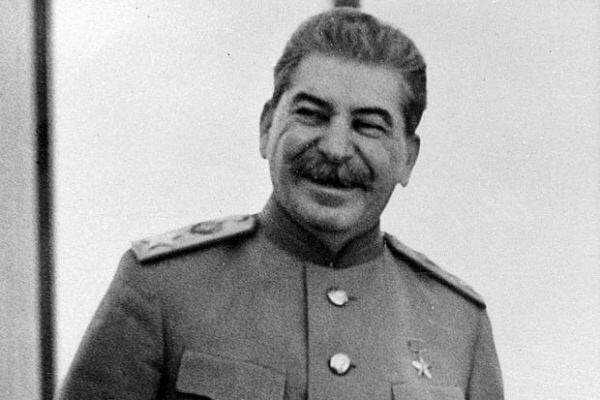
\includegraphics[scale=0.3]{happystalin.jpg}
\end{center}
\end{frame}

\begin{frame}
\frametitle{Why Coq and why not JavaScript ?}
\begin{center}
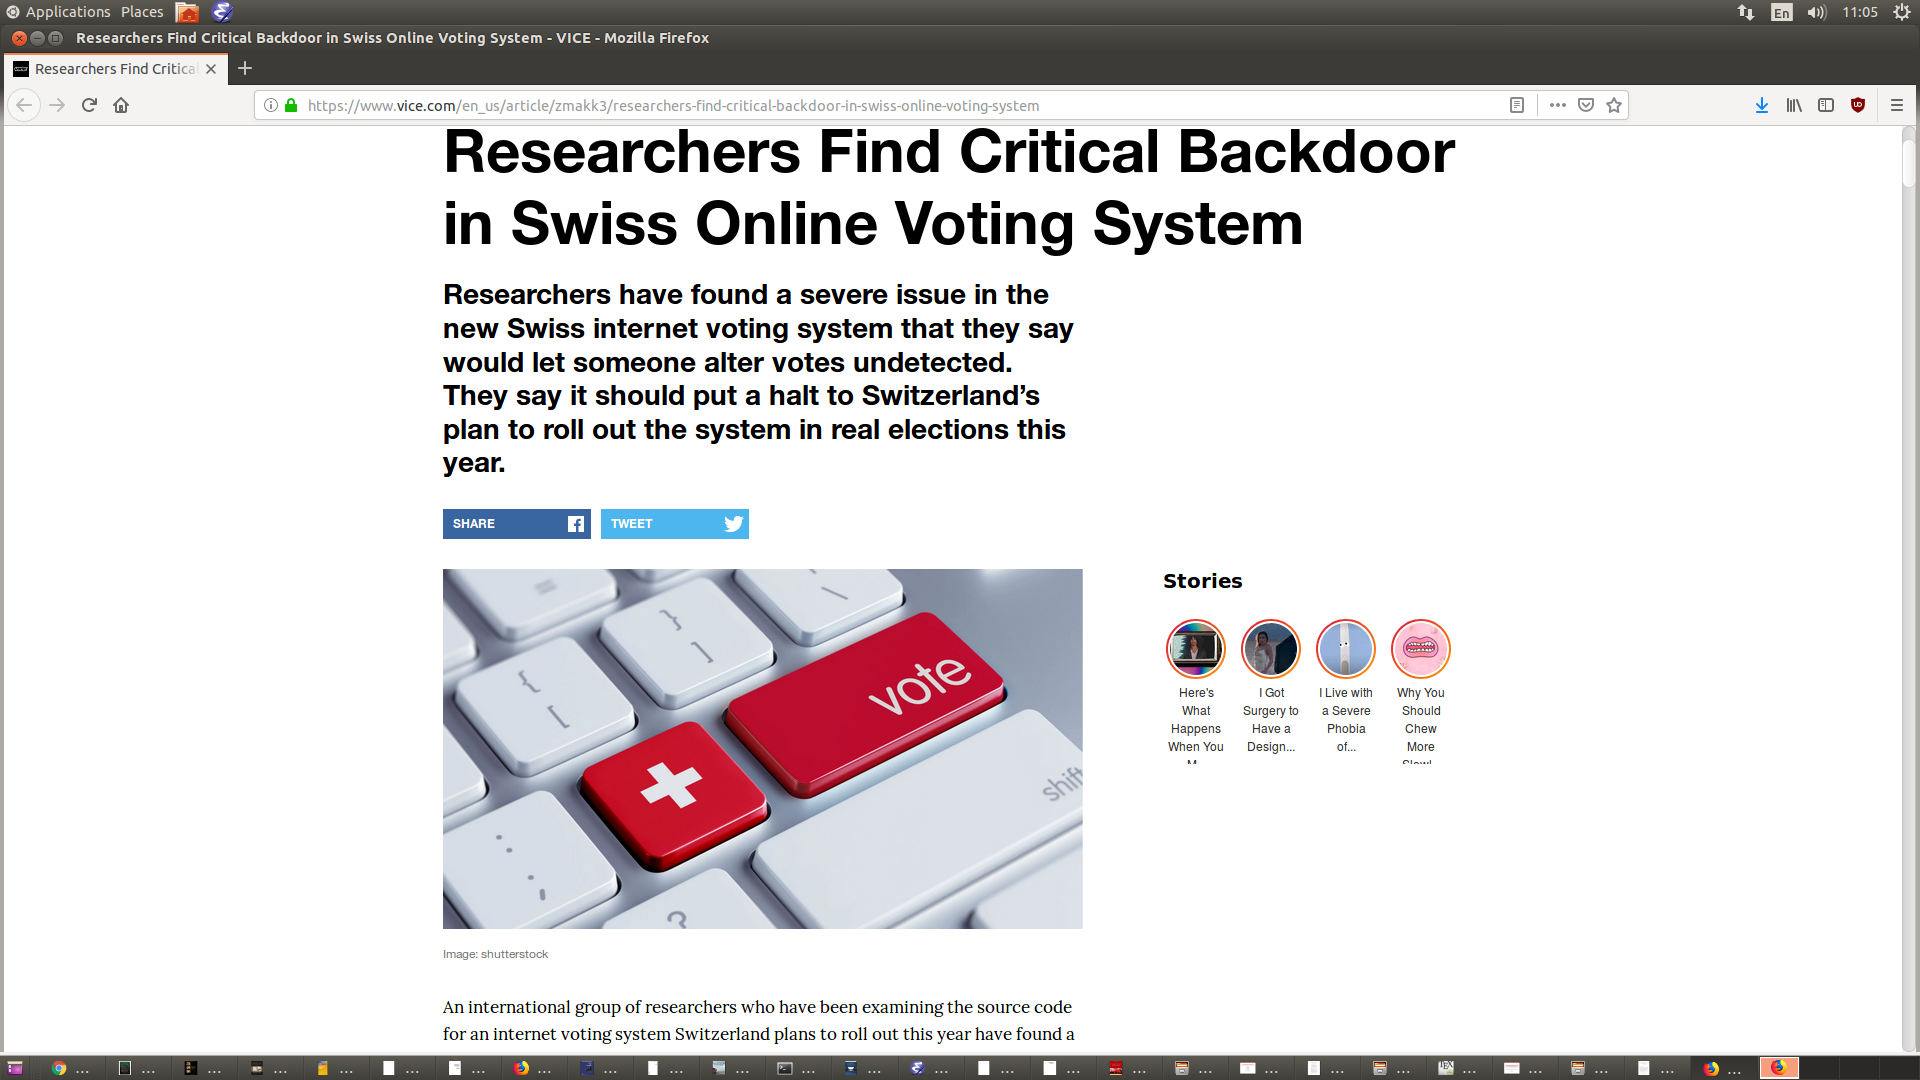
\includegraphics[scale=0.15]{swisspost.png}
\end{center}
\end{frame}

%\begin{frame}
%\frametitle{Why Schulze Method ?}
%\begin{itemize}
%\item De facto standard in many communities over Internet. 
%\item According to Arrow's impossibility theorem, no preferential voting scheme 
%can guarantee all desirable properties, but Schulze method offers good compromise.

% that one would like to impose due to Arrow’s theorem, the Schulze method offers a good compromise, with a number of important properties
%already  established  in  Schulze’s  original  paper, like monotonicity, Condorcet consistency, and Majority.
%\item Although Schulze method is not used in any parliamentary elections, but it's 
%      de facto standard in many communities over Internet. It is used 
%	 used in the elections of almost 60 organization including Free Software Foundation, Gentoo Foundataion, Haskell and Pirate Party of many countries. Part of the reason for its popularity is that no preferential voting scheme can guarantee
%all desirable properties that one would like to impose due to Arrow’s theorem, the Schulze method offers a good compromise, with a number of important properties
%already  established  in  Schulze’s  original  paper, like monotonicity, Condorcet consistency, and Majority.


%\item Gaining popularity in the open source community\pause
%\item Quantative comparison by Rivest and Shen
%\item Lots of good properties e.g. monotonicity, majority, condercet\pause 
%\item Trust in electronic elections using formal verification [ITP 2017]\pause
%\item Case study to demonstrate real world counting [E-Vote-ID 2017]
%\end{itemize}
%\end{frame}


%\begin{frame}
%\frametitle{Schulze Method}
%\begin{itemize}
%\item Collective preferences can be cyclic, even if the preferences of individual voters are not cyclic.
%\end{itemize}
%\begin{figure}[ht]
%\centering
%$
%\xymatrix@R=12ex@C=12ex{
%A \ar@/^/[rr]^{3} \ar@/_/[dr]_{-1} & & B \ar@/^/[ll]^{-3}
%\ar@/^/[dl]^5 \\
%& C \ar@/_/[ul]_{1} \ar@/^/[ur]^{-5}
%}$\end{figure}
%\begin{itemize}
%\item The main idea of the method is to resolve cycles by considering \emph{transitive preferences} or a generalised notion of margin.
%\end{itemize}
%\end{frame}

\begin{frame}
\frametitle{Schulze Method (Plain Text Ballot)}

\begin{itemize}
\item Consider an election with a set of $m$ candidates $C$ = $\{c1,\dots,cm\}$, and 
	a multi-set of $n$ votes $P$ = $\{b1,\dots,bn\}$. A (plaintext) ballot
	is represented as function $b: C \rightarrow \mathbb{N}$ that 
	assigns natural 	number (the preference) to each candidate.

	%\begin{wrapfigure}[14]{r}[0cm]{0.4\textwidth}
  \begin{center}
    %\raisebox{0pt}[-1cm]
    \raisebox{0pt}[\dimexpr\height-0.5\baselineskip\relax]
    {
\includegraphics[width=0.30\textwidth]{bal-cropped.pdf}}
    \raisebox{0pt}[\dimexpr\height-8.5\baselineskip\relax]{}
    %\includegraphics[width=4cm]{ballot.png}
  \end{center}
  %\end{wrapfigure}

\end{itemize}
\end{frame}


\begin{frame}
\frametitle{Schulze Method (Margin Matrix)}
\begin{itemize}

\item Given two candidates $c, d \in C$,
the \emph{margin} of $c$ over $d$ is
the number of voters that prefer $c$ over $d$, minus the number of voters that prefer $d$ over $c$. 
\[
  m(c, d) = \sharp \lbrace b \in P \mid c >_b d \rbrace -
            \sharp \lbrace b \in P \mid d >_b c \rbrace
\] where $\sharp$ denotes cardinality and $>_b$ is the 
ordering given by the ballot $b$.
\end{itemize}
\end{frame}

%\begin{frame}
%\frametitle{Schulze Method}
%\begin{itemize}
%\item Example of Graph G (collective preferences can be cyclic, even if the preferences of individual voters are not cyclic). The main idea of the method is to resolve cycles by considering \emph{transitive preferences} or a generalised notion of margin.
%\[
%\xymatrix@R=12ex@C=12ex{
%A \ar@/^/[rr]^{3} \ar@/_/[dr]_{-1} & & B \ar@/^/[ll]^{-3}
%\ar@/^/[dl]^5 \\
%& C \ar@/_/[ul]_{1} \ar@/^/[ur]^{-5}
%}\]
%\end{itemize}
%\end{frame}


\begin{frame}
\frametitle{Schulze Method (Generalized Margin Matrix)}
\begin{itemize}

\item A directed \emph{path} from
candidate $c$ to candidate $d$ is a sequence $p \equiv c_0, \dots, c_{n+1}$
of candidates with $c_0 = c$ and $c_{n+1} = d$ ($n \geq 0$), and the
\emph{strength}, st, of path, p, is the minimum margin of adjacent
nodes, i.e.
\[ st(c_0, \dots, c_{n+1}) = \min \lbrace m (c_i, c_{i+1}) \mid 0
\leq i \leq n \rbrace. \]\pause
\item For candidates c and d, let $M(c, d)$ denote the maximum strength, or generalized margin of a path
	from c to d i.e. 
	\[ M(c, d) = \max \lbrace st (p) : \text{p is path from c to d in G} \rbrace\]\pause
	
\item The winning set (always non empty) is defined as 
 \[ W =  \lbrace c \in C : \forall d \in C \setminus \{c\}, M (c, d) \geq M (d, c) \rbrace\]

\end{itemize}
\end{frame}



\begin{frame}
\frametitle{Example of Schulze method}
\begin{itemize}
\item Margin matrix
\[
\xymatrix@R=10ex@C=10ex{
A \ar@/^/[rr]^{3} \ar@/_/[dr]_{-1} & & B \ar@/^/[ll]^{-3}
\ar@/^/[dl]^5 \\
& C \ar@/_/[ul]_{1} \ar@/^/[ur]^{-5}
} \] \pause
\item Computing generalized margin
\[\xymatrix@R=10ex@C=10ex{
A \ar@/^/[rr]^{3} \ar@/_/[dr]_{3} & & B \ar@/^/[ll]^{1}
\ar@/^/[dl]^5 \\
& C \ar@/_/[ul]_{1} \ar@/^/[ur]^{1}
}\]
\end{itemize}
\end{frame}

\begin{frame}
\frametitle{A Question to Ponder}

\begin{center}
Can we guess the ballots from Margin matrix ? 

\includegraphics[scale=0.3]{pondering.jpg}
\end{center}
\end{frame}


\begin{frame}
\frametitle{Homomorphic Schulze (Pillars)}
\begin{itemize}
\item Homomorphic Encryption 
\item Zero Knowledge Proof
\end{itemize}

\end{frame}

\begin{frame}
\frametitle{Ballot Representation for Homomorphic Schulze}
\begin{itemize}
\item Plaintext ballot 
$$\bordermatrix{\text{}& Dirk & Mina & Caity \cr
                Dirk & 0 &  1 & 1\cr
                Mina & -1 &  0 & 1\cr
                Caity & -1 &  -1 & 0}$$ \pause
  
\item Ciphertext ballot 
  $$\bordermatrix{\text{}& Dirk & Mina & Caity \cr
                Dirk & (42.., 15..) & (63.., 54..) & (89.., 67..)\cr
                Mina & (16.., 43..) & (12.., 46..) & (71.., 11..)\cr
                Caity & (96.., 67..) & (54.., 43..) & (39.., 28..)}$$
 
  \end{itemize}
\end{frame}


\begin{frame}
\frametitle{Homomorphic Margin Computation}
\begin{itemize}
 \item Margin from plaintext ballots 
    \[ m(c, d) = \sum_{b \in B} b(x, y) \]\pause

 \item Encrypted margin from ciphertext ballots
      \[ encm(c, d) = \bigoplus_{encb \in EncB} encb(x, y) \] \pause
      
 \item In additive Elgamal encryption, $E(m) = (g^r, g^m * h^r)$. We can easily 
  	verify that $E(m_{1}) * E(m_{2}) = E (m_{1} + m_{2})$.     
\end{itemize}

\end{frame}

\begin{frame}
\frametitle{Problems with Matrix Representation}
\begin{itemize}
\item Voter can inflate your ballot
$$\bordermatrix{\text{}& Dirk & Mina & Caity \cr
                Dirk & 0 &  10 & 10\cr
                Mina & -10 &  0 & 10\cr
                Caity & -10 &  -10 & 0}$$ \pause
         
\item Voter can construct cyclic ballot
$$\bordermatrix{\text{}& Dirk & Mina & Caity \cr
                Dirk & 0 &  1 & 0\cr
                Mina & -1 &  0 & 1\cr
                Caity & 1 & -1 & 0}$$
                
\end{itemize}
                
\end{frame}

\begin{frame}
\frametitle{Solution (Protocol Design)}
\begin{itemize}
\item We take a ballot (u)
$$\bordermatrix{\text{}& Dirk & Mina & Caity \cr
                Dirk & (42.., 15..) & (63.., 54..) & (89.., 67..)\cr
                Mina & (16.., 43..) & (12.., 46..) & (71.., 11..)\cr
                Caity & (96.., 67..) & (54.., 43..) & (39.., 28..)}$$ \pause
              
\item We generate a secret random 
	  permutation, $\sigma$, publish its commitment, 
	  and zero knowledge proof. \pause

\item We permute each row of ballot u by $\sigma$ which produces row-shuffled
      ballot (v) and zero knowledge proof 
 $$\bordermatrix{\text{}& Dirk & Mina & Caity \cr
                Dirk & (36.., 97..) & (81.., 51..) & (12.., 98..)\cr
                Mina & (31.., 23..) & (78.., 67..) & (19.., 41..)\cr
                Caity & (76.., 44..) & (31.., 61..) & (43.., 22..)}$$ 
\end{itemize}
\end{frame} 

\begin{frame}
\frametitle{Solution (Protocol Design)}
\begin{itemize}
\item We permute each column of ballot v by $\sigma$ (w) in similar fashion   
 $$\bordermatrix{\text{}& Dirk & Mina & Caity \cr
                Dirk & (31.., 44..) & (73.., 35..) & (43.., 65..)\cr
                Mina & (82.., 36..) & (56.., 82..) & (27.., 23..)\cr
                Caity & (67.., 38..) & (15.., 91..) & (89.., 98..)}$$ 

\item We decrypt the encrypted ballot w into plain text ballot b with 
	  zero knowledge proof that b is indeed honest decryption of w.

\end{itemize}
\end{frame}

%
%\begin{frame}
%\frametitle{Computation of generalized margin}
%%\begin{itemize}
%\genmargin
%%\end{itemize}
%\end{frame}
%

%\begin{frame}
%\frametitle{Computation of generalized margin}
%\begin{center}
%Cheers. We are done!
%\end{center}
%\begin{center}
%
\includegraphics[scale=0.3]{cheers.jpg}
%\end{center}
%\end{frame}
%
%\begin{frame}
%\frametitle{Computation of generalized margin}
%\begin{itemize}
%\item How do we know that when M stabilises ? 
%\end{itemize}
%\end{frame}
%
%
%\begin{frame}
%\frametitle{Scrutiny Sheet}
%\begin{itemize}
%
%\item One major aspect of our work is that we are not only computing the set of winners, but in fact presenting
%\emph{evidence} for the fact that a particular
%candidate does or does not win. In the context of electronic vote counting, this is known as a \emph{scrutiny sheet}: a tabulation of all relevant data that allows
%us to verify the election outcome.
%
%\end{itemize}
%\end{frame}
%
%\begin{frame}
%\frametitle{Scrutiny Sheet}
%\lstnineth
%\end{frame}
%
%\begin{frame}
%\frametitle{Coq formalization}
%\begin{itemize}
%\item To demonstrate that a candidate $c$ wins, we need to exhibit an integer
%$k$ for all competitors $d$, together with
%\begin{itemize}
%  \item evidence for the existence of a path from $c$ to $d$ with
%  strength $\geq k$ 
%  \item evidence for the non-existence of a path from $d$ to $c$
%  that is stronger than $k$
%\end{itemize}
%\item The first item is straight forward, as a path itself is evidence for the existence of a path, and the notion of path is inductively defined. 
%\item For the second item, we need to produce evidence of membership in the complement of an inductively
%defined set (Coinduction).
%\end{itemize}
%\end{frame}
%
%\begin{frame}
%\frametitle{Coq formalization}
%\begin{itemize}
%\item Mathematically, given $k \in Z$ and a margin function $m: C \times C
%\to Z$, the pairs $(c, d) \in C \times C$ for which there exists a
%path of strength $\geq k$ that joins both are precisely the elements
%of the least fixpoint $LFP(V_k)$ of the monotone operator $V_k: Pow(C \times C) \to Pow(C \times C)$, defined by
%\begin{align}
%V_k(R) = \lbrace& (c, e) \in C^2 \mid m(c, e) \geq k \mbox{ or } \nonumber  \\
%    &(m(c, d) \geq k \mbox{ and } (d, e) \in R \mbox{ for some }  d \in C) \rbrace.\nonumber 
%\end{align}
%%It is easy to see that this operator is indeed monotone, and that
%%the least fixpoint exists, e.g. using Kleene's theorem.  To show that there is \emph{no}
%%path between $d$ and $c$ of strength $> k$, we therefore need to
%%establish that
%%$(d, c) \notin LFP(V_{k+1})$.
%
%\end{itemize}
%\end{frame}
%
%\begin{frame}
%\frametitle{Coq formalization}
%\lstf
%\end{frame}
%
%
%\begin{frame}
%\frametitle{Coq formalization}
%\begin{itemize}
%\item %It is easy to see that this operator is indeed monotone, and that
%%the least fixpoint exists, e.g. using Kleene's theorem.  
%To show that there is \emph{no}
%path between $d$ and $c$ of strength $> k$, we therefore need to
%establish that
%$(d, c) \notin LFP(V_{k+1})$.
%
%\item By duality between least and greatest fixpoints, we have that \[
%(c, d) \in C \times C
%\setminus LFP(V_{k+1}) \iff (c,d) \in GFP(W_{k+1}) \]
%where for arbitrary $k$, $W_k: Pow(C \times C) \to Pow(C \times C)$ is the operator dual
%to $V_k$, i.e.
%\[ W_k(R) = C \times C \setminus (V_k (C\times C \setminus R)) \]
%and $GFP(W_k)$ is the greatest fixpoint of $W_k$. 
%\item As a consequence, to demonstrate that there is \emph{no} path of
%strength $\geq k$ between candidates $d$ and $c$, we need to
%demonstrate that $(d, c) \in GFP(W_{k+1})$.
%
%\end{itemize}
%\end{frame}
%
%\begin{frame}
%\frametitle{Coq formalization}
%\begin{itemize}
%\item %By the Knaster-Tarski fixpoint
%%theorem, this greatest fixpoint is the supremum of all
%%$W_{k+1}$-coclosed sets, that is, sets $R \subseteq C \times C$ for which
%%$R \subseteq W_{k+1}(R)$.
%%That is, 
%To demonstrate that $(d, c) \in GFP(W_{k+1})$, we need
%to exhibit a $W_{k+1}$-coclosed set $R$ with $(d, c) \in R$.
%\begin{align}
%W_k(R) = \lbrace& (c, e) \in C^2 \mid m(c, e) < k \mbox { and} \nonumber \\
% &(m(c, d) < k \mbox{ or } (d,e) \in R \mbox{ for all } d \in C)
%\rbrace \nonumber
%\end{align}
%\end{itemize}
%\end{frame}
%
%%\begin{frame}
%%\frametitle{Coq formalization of Path (Prop Level)}
%%\lstf
%%\end{frame}
%
%\begin{frame}
%\frametitle{Coq formalization}
%\lsts
%\end{frame}
%
%\begin{frame}
%\frametitle{Coq formalization}
%\lstt
%\end{frame}
%
%\begin{frame}
%\frametitle{Coq formalization}
%\begin{itemize}
%\item The proof of the first statement is completely straightforward, as
%the type carries all the information needed to establish the
%propositional winning condition. For the second statement above, we
%introduce an intermediate lemma based on the \emph{iterated margin
%function} $M_k: C \times C \to \mathbb{Z}$. Intuitively, $M_k (c, d)$ is the
%strength of the strongest path between $c$ and $d$ of length $\leq
%k+1$. 
%\begin{align}
%&M_0 (c, d) = m(c, d) \nonumber \\
%&M_{i+1}(c, d) = \max \lbrace M_i(c, d), \max \lbrace  \min
%\lbrace m(c, e), M_i(e, d) \mid e \in C \rbrace \rbrace \rbrace \nonumber
%\end{align}
%
%
%\end{itemize}
%\end{frame}
%
%
%\begin{frame}
%\frametitle{Coq formalization}
%\begin{itemize}
%\item We establish this fact that
%paths with repeated nodes do not  contribute to the maximal strength of a
%path. Therefore, the iterated margin function stabilises at the $n$-th iteration
%(where $n$ is the number of candidates).
%\lsteleven
%
%\end{itemize}
%\end{frame}

%\begin{frame}
%\frametitle{Schulze Method}
%\begin{itemize}
%\item Compute the \emph{margin function} $m(c, d)$ as the number of
%ballots that strictly prefer $c$ over $d$, minus the number of
%ballots that strictly prefer $d$ over $c$\pause
%\item Compute the \emph{generalised margin function} $g(c, d)$ as
%the maximal path-based margin between $c$ and $d$\pause
%\item Compute winning candidate, i.e. candidates for which $g(c, d)
%\geq g(c, d)$, for all other candidates $d$, and apply tie-breaking
%if more than one winning candidate has been elected.
%\end{itemize}
%\end{frame}


%\begin{frame}
%\frametitle{Formal specification of Schulze method (Prop Level)}
%\lstf
%\end{frame}


%\begin{frame}
%\frametitle{Formal specification of Schulze method (Type Level)}
%\lstt
%\end{frame}

%\begin{frame}
%\frametitle{Formal specification of Schulze method (Type Level)}
%\begin{itemize}
%\item $W_{k} (S) $ = $ \{(a, b) \mid \text{margin a b $<$ k } \land \text{ }
%            (\forall m, \text{ margin a m $<$ k } 
%            \lor (m, b) \in S)\}$\pause
%\item $Coclosed_{k} (S) $ = $ S \subseteq W_{k} (S) $\pause
%\item $ S \subseteq W_{k}(S) \implies S \subseteq gfp(W_{k}(S)) $ by Knaster-Tarski fixpoint theorem\pause
%\end{itemize}
%\lsts
%\end{frame}

%\begin{frame}
%\begin{itemize}
%\item A ballot is a linear preorder over the set of candidates.\pause
%\end{itemize}
%\begin{center}
%{
\includegraphics[scale=0.20]{bal-cropped.pdf}}
%\end{center}
%\end{frame}
%
%\begin{frame}
%\frametitle{Counting ballots}
%\lstfourth
%\end{frame}
%
%\begin{frame}
%\frametitle{All Schulze Election Have Winners}
%  \lsttwelve
%\end{frame}
%
%\begin{frame}
%\frametitle{Scrutiny Sheet}
%\begin{itemize}
%
%\item One major aspect of our work is that we are not only computing the set of winners, but in fact presenting
%\emph{evidence} for the fact that a particular
%candidate does or does not win. In the context of electronic vote counting, this is known as a \emph{scrutiny sheet}: a tabulation of all relevant data that allows
%us to verify the election outcome.
%
%\end{itemize}
%\end{frame}
%
%\begin{frame}
%\frametitle{Scrutiny Sheet}
%\lstnineth
%\end{frame}

%\begin{frame}
%\frametitle{Certificate}
%\lstfifth
%\end{frame}

\begin{frame}
\frametitle{Experimental Result}
{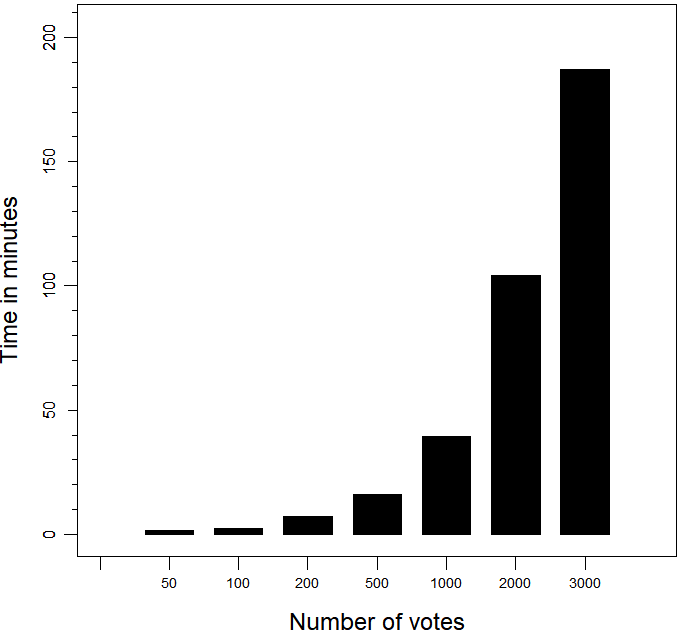
\includegraphics[scale=0.40]{PlotVer3.png}}
\end{frame}



%\begin{frame}
%\frametitle{In Previous Presentation}
%\begin{itemize}
%\item Exploring the avenues of cryptography [July 2017 - December 2017]
%\item Risk limiting audit [January 2018 - June 2018]
%\item Connecting it with Helios [July 2018 - December 2018]
%\item Thesis writing [January 2019 - June 2019]
%\end{itemize}
%
%\end{frame}

%% New addition for september presentation
%\begin{frame}
%\frametitle{Pros and Cons}
%\begin{itemize}
%\item Counting on plaintext ballots offers universal verifiability, meaning
%	  that anyone can check that the announced tally is correct based on certificate 
%	  we publish, but at the same time it opens the door of coercion (Italian attack).
%\item Can we achieve better way to count the ballots without revealing 	
%	the content posted on bulletin board ? Is it possible to convince the voter 
%	that we (Electoral Authority) have 
%	counted all the ballots honestly i.e we have included all the valid ballots 
%    and excluded all the invalid ballot in counting without revealing the content
%    of ballot itself ? \pause
%
%\item The answer is fortunately yes! Welcome to homomorphic encryption and zero 
%	knowledge proof.
%
%\end{itemize} 
%\end{frame}

%
%\begin{frame}
%\frametitle{Homomorphic Encryption and Zero Knowledge Proof}
%\begin{itemize}
%\item Homomorphic encryption is a form of encryption that allows computations to be carried out on ciphertext and generating an encrypted result. When encrypted result
%is decrypted, it matches the result of operations performed on the plaintext. 
%\item In additive Elgamal encryption, $E(m) = (g^r, g^m * h^r)$. We can easily 
%  	verify that $E(m_{1}) * E(m_{2}) = E (m_{1} + m_{2})$. 
%\item A zero-knowledge protocol is a method by which one party (the prover) can prove to another party (the verifier) that a given statement is true, without conveying any information apart from the fact that the statement is indeed true.
%\end{itemize} 
%\end{frame}
%
%
%\begin{frame}
%\frametitle{Zero Knowledge Proof (Chaum Pedersen)}
%\begin{itemize}
%\item Given group generator g, public key y, plaintext m, and ciphertext 
%	($\alpha$, $\beta$). How would you (Prover) convince me (Challenger) 
%	that m is honest decryption of 
%	($\alpha$, $\beta$) i.e. you hold the private key, x, corresponding to 
%	public key y.
%\item Prover sends $a = g ^ w$, $b = \alpha ^ w$ for random w to Challenger
%\item Challenger computes c = hash (a, b) and sends (c, b) to Prover
%\item Prover sends $ t = w + x * c $
%\item Challenger will verify that $g^t = a * y^c $
%        and $\alpha^t = b * \beta/m ^ c$
%\end{itemize} 
%\end{frame}


%\begin{frame}
%\frametitle{Zero Knowledge Proof (Chaum Pedersen)}
%\deczkp
%\end{frame}
%
%\begin{frame}
%\frametitle{Ballot Representation}
%\begin{itemize}
%\item The new representation of ballot is matrix. \newline
%      Definition pballot := cand $\rightarrow$ cand $\rightarrow$ Z
%      \[  
%  \begin{bmatrix}
%    x_{11}       & x_{12} & x_{13} & \dots & x_{1n} \\
%    x_{21}       & x_{22} & x_{23} & \dots & x_{2n} \\
%    \hdotsfor{5} \\
%    x_{n1}       & x_{n2} & x_{n3} & \dots & x_{nn}
%\end{bmatrix}\]
%      Definition eballot := cand $\rightarrow$ cand $\rightarrow$ Z * Z \newline 
%\[  
%  \begin{bmatrix}
%    (y_{11}, z_{11}) & (y_{12}, z_{12}) & (y_{13}, z_{13}) & \dots & (y_{1n}, z_{1n}) \\
%    (y_{21}, z_{21}) & (y_{22}, z_{22}) & (y_{23}, z_{23}) & \dots & (y_{2n}, z_{2n}) \\
%    \hdotsfor{5} \\
%    (y_{n1}, z_{n1}) & (y_{n2}, z_{n2}) & (y_{n3}, z_{n3}) & \dots & (y_{nn}, z_{nn})
%\end{bmatrix}\] 	 
%\item  we do point wise
%	multiplication of two encrypted ballots (matrices) to achieve the goal 
%	of addition in 	plain text. 
%	
%
%\end{itemize} 
%\end{frame}
%
%\begin{frame}
%\frametitle{Ballot Validity}
%\begin{itemize}
%\item A ballot is valid if all the entries are -1, 0 or 1, and it has no
%	cycle. If voter prefers candidate $A$ over $B$ then it marks 1 in row 
%	$A$ and column $B$, and -1 in row $B$ and column $A$. No one is preferred over
%	itself so all the diagonal entries are 0.  
%
%\end{itemize}
%\matvalid
%\end{frame}	
%
%
%
%
%
%\begin{frame}
%\frametitle{Challenge}
%\begin{itemize}
%
%\item A malicious 
%	user can mark ballot in such a way that it might lead to cycle, or inflate the 
%	ballot.
%\item The challenge in the counting process is  convincing the malicious user 
%	that your vote is invalid and discarded in final counting without decrypting 
%	his ballot, and convincing honest user that your vote is valid and included in 
%	final counting without decrypting his ballot.  
%
%\end{itemize}
%
%\end{frame}
%
%\begin{frame}
%\frametitle{Zero Knowledge Proof Primitives}
%\begin{itemize}
%
%\item Zero knowledge proof of decryption
%\item Zero knowledge proof of (secret) permutation
%\item Zero knowledge proof of shuffle  
%
%\end{itemize}
%\end{frame}
%
%
%\begin{frame}
%
%\frametitle{Protocol Design}
%\begin{itemize}
%\item We generate a secret permutation, $\sigma$, commit it, and prove under 
%      zero knowledge that commitment contains indeed a permutation matrix.
%\item We pass the each encrypted ballot, u, through mix nets (secret permutation
% function) $\sigma$, which permutes the each row of ballot, u, producing ballot, v, with 
% zero knowledge proof that each row of v is indeed a permutation of each row u, 
% and permute each column of v by same secret permutation $\sigma$ producing ballot,
% w, with zero knowledge proof that each column of w is indeed a permutation of 
% each column of v. 
%  
%\item We decrypt the encrypted ballot w into plain text ballot b with zero knowledge 
%      proof that b is indeed honest decryption of w. We have formally 
% established that if b is valid (i.e. each entry is -1, 0 or 1, and there is no
% cycle) then ballot u is also valid.
%
%\end{itemize}
%\end{frame}
%
%\begin{frame}
%\frametitle{Axioms used in formalization}
%\axiomone
%\end{frame}
%
%\begin{frame}
%\frametitle{Axioms used in formalization}
%\axiomtwo
%\end{frame}

%\begin{frame}
%\frametitle{Computation as Inductive data type}
%\lstseventeen
%\end{frame}

%\begin{frame}
%\frametitle{Computation as Inductive data type}
%\lstthirteen
%\end{frame}
%
%%\begin{frame}
%%\frametitle{Computation as Inductive data type}
%%\lstfourteen
%%\end{frame}
%
%\begin{frame}
%\frametitle{Computation as Inductive data type}
%\lstfifteen
%\end{frame}
%
%\begin{frame}
%\frametitle{Computation as Inductive data type}
%\lstsixteen
%\end{frame}
%
%
%\begin{frame}
%\frametitle{Proof of correctness}
%\proofcorrectness
%\end{frame}

%\begin{frame}
%\frametitle{Future Work}
%\begin{itemize}
%\item Finish the current project
%\item Risk limiting audit [June 2018 - December 2018]
%\item Proving the properties of Schulze Method [Jan 2019 - July 2019]
%\item Thesis writing [July 2019 - December 2019]
%\end{itemize}
%
%\end{frame}
%
%\begin{frame}
%\frametitle{Future Work}
%\begin{itemize}
%\item I am running 6 month behind my estimation :(.
%\item Finish the current project (Finished)
%\item Risk limiting audit [June 2018 - December 2018]
%\item Proving the properties of Schulze Method [Jan 2019 - July 2019]
%\item Thesis writing [July 2019 - December 2019]
%\end{itemize}
%\end{frame}

\begin{frame}
\begin{center}
{\fontsize{40}{50}\selectfont Thank You!}
{
\includegraphics[scale=0.05]{turbo.jpg}}
\end{center}
\end{frame}



\end{document}
